\documentclass[tikz,border=6pt]{standalone}
\usepackage{tikz}
\begin{document}
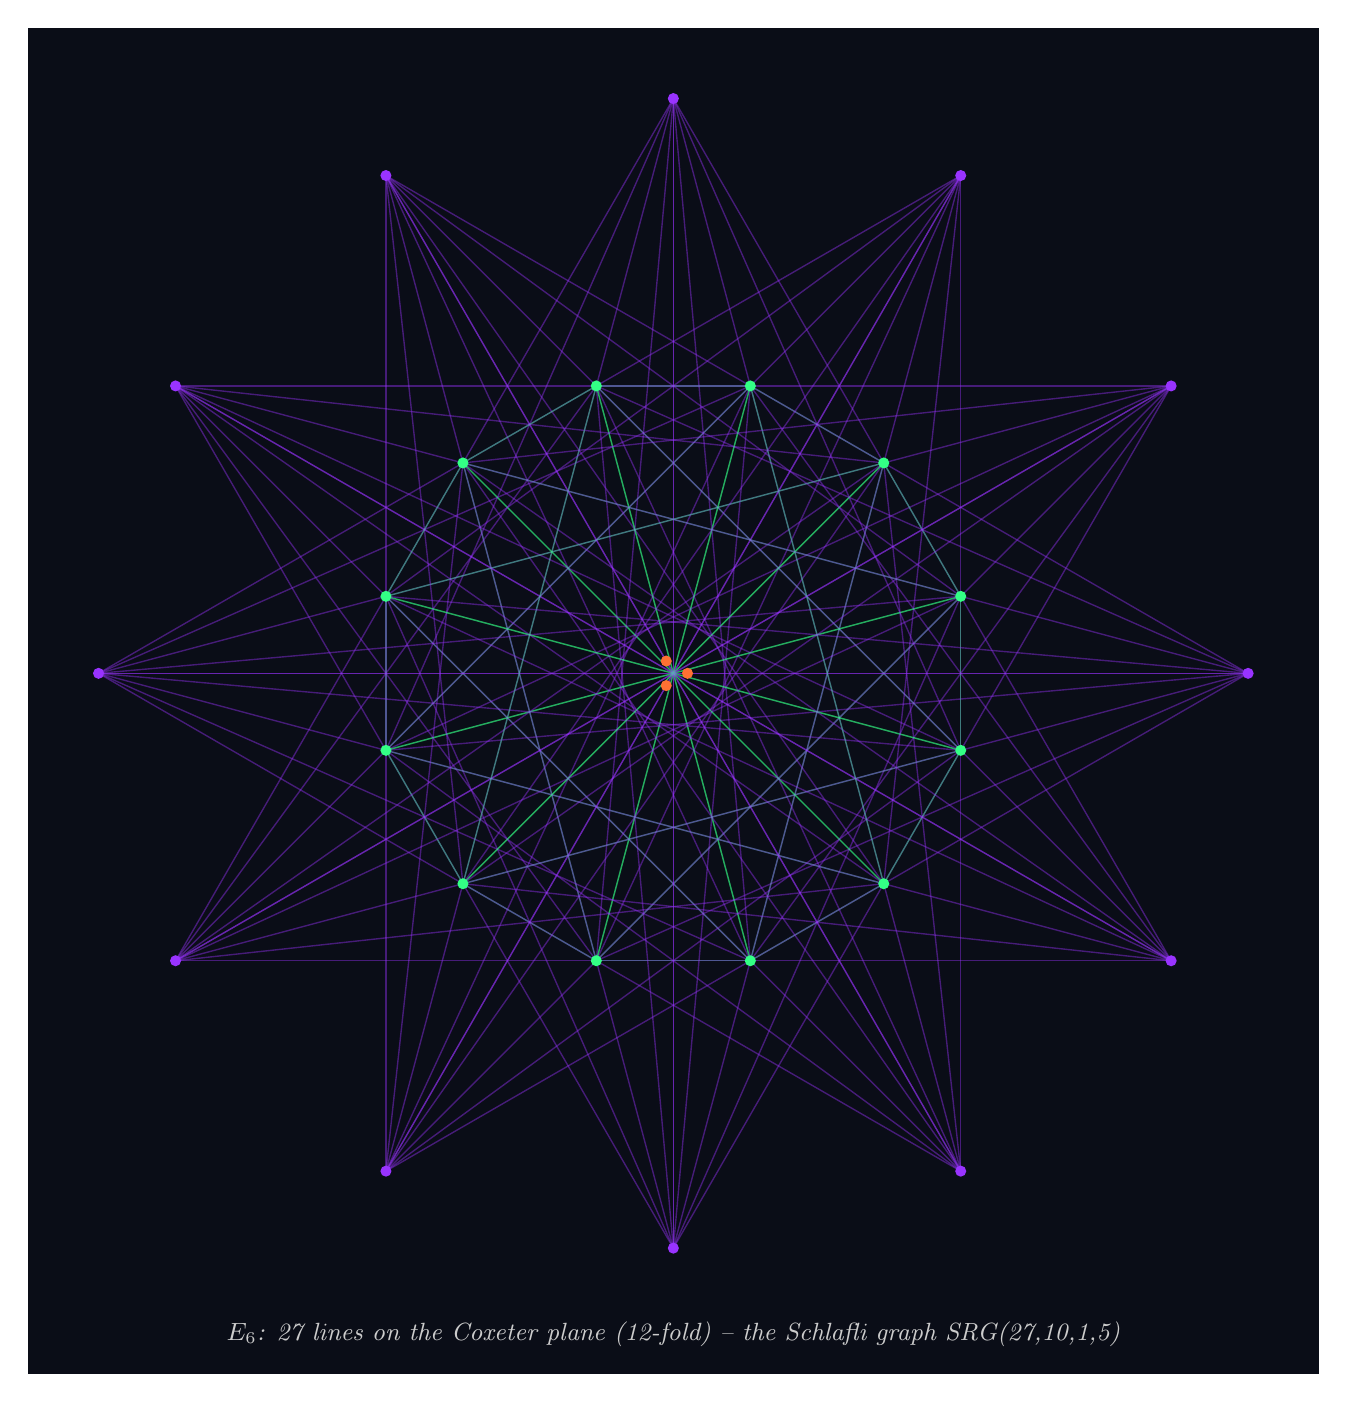
\begin{tikzpicture}
\definecolor{ring0}{rgb}{1.000,0.440,0.200}
\definecolor{ring1}{rgb}{0.200,1.000,0.520}
\definecolor{ring2}{rgb}{0.600,0.200,1.000}
\definecolor{bg}{rgb}{0.04,0.05,0.09}
\fill[bg] (-8.2,-8.9) rectangle (8.2,8.2);
\draw[ring1,line width=0.5pt,opacity=0.42] (-0.978,-3.650)--(0.978,-3.650);
\draw[ring2,line width=0.5pt,opacity=0.42] (-0.978,-3.650)--(-0.000,7.300);
\draw[ring1,line width=0.5pt,opacity=0.42] (-0.978,-3.650)--(0.000,0.000);
\draw[ring1,line width=0.5pt,opacity=0.42] (-0.978,-3.650)--(-2.672,2.672);
\draw[ring1,line width=0.5pt,opacity=0.42] (-0.978,-3.650)--(-2.672,-2.672);
\draw[ring2,line width=0.5pt,opacity=0.42] (-0.978,-3.650)--(7.300,0.000);
\draw[ring2,line width=0.5pt,opacity=0.42] (-0.978,-3.650)--(-6.322,3.650);
\draw[ring2,line width=0.5pt,opacity=0.42] (-0.978,-3.650)--(3.650,6.322);
\draw[ring1,line width=0.5pt,opacity=0.42] (-0.978,-3.650)--(3.650,0.978);
\draw[ring1,line width=0.5pt,opacity=0.42] (-0.978,-3.650)--(0.978,3.650);
\draw[ring2,line width=0.5pt,opacity=0.42] (0.978,-3.650)--(-0.000,7.300);
\draw[ring2,line width=0.5pt,opacity=0.42] (0.978,-3.650)--(-7.300,-0.000);
\draw[ring1,line width=0.5pt,opacity=0.42] (0.978,-3.650)--(2.672,2.672);
\draw[ring1,line width=0.5pt,opacity=0.42] (0.978,-3.650)--(2.672,-2.672);
\draw[ring1,line width=0.5pt,opacity=0.42] (0.978,-3.650)--(-0.000,-0.000);
\draw[ring1,line width=0.5pt,opacity=0.42] (0.978,-3.650)--(-0.978,3.650);
\draw[ring2,line width=0.5pt,opacity=0.42] (0.978,-3.650)--(-3.650,6.322);
\draw[ring1,line width=0.5pt,opacity=0.42] (0.978,-3.650)--(-3.650,0.978);
\draw[ring2,line width=0.5pt,opacity=0.42] (0.978,-3.650)--(6.322,3.650);
\draw[ring2,line width=0.5pt,opacity=0.42] (0.000,-7.300)--(-0.000,0.000);
\draw[ring2,line width=0.5pt,opacity=0.42] (0.000,-7.300)--(-0.000,7.300);
\draw[ring2,line width=0.5pt,opacity=0.42] (0.000,-7.300)--(-0.978,3.650);
\draw[ring2,line width=0.5pt,opacity=0.42] (0.000,-7.300)--(-3.650,6.322);
\draw[ring2,line width=0.5pt,opacity=0.42] (0.000,-7.300)--(-3.650,0.978);
\draw[ring2,line width=0.5pt,opacity=0.42] (0.000,-7.300)--(6.322,3.650);
\draw[ring2,line width=0.5pt,opacity=0.42] (0.000,-7.300)--(-6.322,3.650);
\draw[ring2,line width=0.5pt,opacity=0.42] (0.000,-7.300)--(3.650,6.322);
\draw[ring2,line width=0.5pt,opacity=0.42] (0.000,-7.300)--(3.650,0.978);
\draw[ring2,line width=0.5pt,opacity=0.42] (0.000,-7.300)--(0.978,3.650);
\draw[ring2,line width=0.5pt,opacity=0.42] (-0.000,0.000)--(-0.000,7.300);
\draw[ring2,line width=0.5pt,opacity=0.42] (-0.000,0.000)--(-7.300,-0.000);
\draw[ring1,line width=0.5pt,opacity=0.42] (-0.000,0.000)--(2.672,2.672);
\draw[ring1,line width=0.5pt,opacity=0.42] (-0.000,0.000)--(2.672,-2.672);
\draw[ring0,line width=0.5pt,opacity=0.42] (-0.000,0.000)--(-0.000,-0.000);
\draw[ring0,line width=0.5pt,opacity=0.42] (-0.000,0.000)--(0.000,0.000);
\draw[ring1,line width=0.5pt,opacity=0.42] (-0.000,0.000)--(-2.672,2.672);
\draw[ring1,line width=0.5pt,opacity=0.42] (-0.000,0.000)--(-2.672,-2.672);
\draw[ring2,line width=0.5pt,opacity=0.42] (-0.000,0.000)--(7.300,0.000);
\draw[ring2,line width=0.5pt,opacity=0.42] (-3.650,-0.978)--(3.650,-6.322);
\draw[ring2,line width=0.5pt,opacity=0.42] (-3.650,-0.978)--(-0.000,7.300);
\draw[ring1,line width=0.5pt,opacity=0.42] (-3.650,-0.978)--(2.672,-2.672);
\draw[ring1,line width=0.5pt,opacity=0.42] (-3.650,-0.978)--(-0.000,-0.000);
\draw[ring1,line width=0.5pt,opacity=0.42] (-3.650,-0.978)--(-3.650,0.978);
\draw[ring2,line width=0.5pt,opacity=0.42] (-3.650,-0.978)--(6.322,3.650);
\draw[ring1,line width=0.5pt,opacity=0.42] (-3.650,-0.978)--(-2.672,-2.672);
\draw[ring2,line width=0.5pt,opacity=0.42] (-3.650,-0.978)--(7.300,0.000);
\draw[ring1,line width=0.5pt,opacity=0.42] (-3.650,-0.978)--(3.650,0.978);
\draw[ring1,line width=0.5pt,opacity=0.42] (-3.650,-0.978)--(0.978,3.650);
\draw[ring2,line width=0.5pt,opacity=0.42] (3.650,-6.322)--(-0.000,7.300);
\draw[ring2,line width=0.5pt,opacity=0.42] (3.650,-6.322)--(-7.300,-0.000);
\draw[ring2,line width=0.5pt,opacity=0.42] (3.650,-6.322)--(2.672,2.672);
\draw[ring2,line width=0.5pt,opacity=0.42] (3.650,-6.322)--(-0.978,3.650);
\draw[ring2,line width=0.5pt,opacity=0.42] (3.650,-6.322)--(-3.650,6.322);
\draw[ring2,line width=0.5pt,opacity=0.42] (3.650,-6.322)--(0.000,0.000);
\draw[ring2,line width=0.5pt,opacity=0.42] (3.650,-6.322)--(-2.672,2.672);
\draw[ring2,line width=0.5pt,opacity=0.42] (3.650,-6.322)--(-6.322,3.650);
\draw[ring2,line width=0.5pt,opacity=0.42] (3.650,-6.322)--(3.650,6.322);
\draw[ring2,line width=0.5pt,opacity=0.42] (-3.650,-6.322)--(3.650,-0.978);
\draw[ring2,line width=0.5pt,opacity=0.42] (-3.650,-6.322)--(-0.000,7.300);
\draw[ring2,line width=0.5pt,opacity=0.42] (-3.650,-6.322)--(2.672,2.672);
\draw[ring2,line width=0.5pt,opacity=0.42] (-3.650,-6.322)--(-0.000,-0.000);
\draw[ring2,line width=0.5pt,opacity=0.42] (-3.650,-6.322)--(-3.650,6.322);
\draw[ring2,line width=0.5pt,opacity=0.42] (-3.650,-6.322)--(6.322,3.650);
\draw[ring2,line width=0.5pt,opacity=0.42] (-3.650,-6.322)--(-2.672,2.672);
\draw[ring2,line width=0.5pt,opacity=0.42] (-3.650,-6.322)--(7.300,0.000);
\draw[ring2,line width=0.5pt,opacity=0.42] (-3.650,-6.322)--(3.650,6.322);
\draw[ring2,line width=0.5pt,opacity=0.42] (-3.650,-6.322)--(0.978,3.650);
\draw[ring2,line width=0.5pt,opacity=0.42] (3.650,-0.978)--(-0.000,7.300);
\draw[ring2,line width=0.5pt,opacity=0.42] (3.650,-0.978)--(-7.300,-0.000);
\draw[ring1,line width=0.5pt,opacity=0.42] (3.650,-0.978)--(2.672,-2.672);
\draw[ring1,line width=0.5pt,opacity=0.42] (3.650,-0.978)--(-0.978,3.650);
\draw[ring1,line width=0.5pt,opacity=0.42] (3.650,-0.978)--(-3.650,0.978);
\draw[ring1,line width=0.5pt,opacity=0.42] (3.650,-0.978)--(0.000,0.000);
\draw[ring1,line width=0.5pt,opacity=0.42] (3.650,-0.978)--(-2.672,-2.672);
\draw[ring2,line width=0.5pt,opacity=0.42] (3.650,-0.978)--(-6.322,3.650);
\draw[ring1,line width=0.5pt,opacity=0.42] (3.650,-0.978)--(3.650,0.978);
\draw[ring2,line width=0.5pt,opacity=0.42] (-6.322,-3.650)--(6.322,-3.650);
\draw[ring2,line width=0.5pt,opacity=0.42] (-6.322,-3.650)--(-0.000,7.300);
\draw[ring2,line width=0.5pt,opacity=0.42] (-6.322,-3.650)--(2.672,2.672);
\draw[ring2,line width=0.5pt,opacity=0.42] (-6.322,-3.650)--(2.672,-2.672);
\draw[ring2,line width=0.5pt,opacity=0.42] (-6.322,-3.650)--(-0.978,3.650);
\draw[ring2,line width=0.5pt,opacity=0.42] (-6.322,-3.650)--(6.322,3.650);
\draw[ring2,line width=0.5pt,opacity=0.42] (-6.322,-3.650)--(0.000,0.000);
\draw[ring2,line width=0.5pt,opacity=0.42] (-6.322,-3.650)--(7.300,0.000);
\draw[ring2,line width=0.5pt,opacity=0.42] (-6.322,-3.650)--(3.650,6.322);
\draw[ring2,line width=0.5pt,opacity=0.42] (-6.322,-3.650)--(3.650,0.978);
\draw[ring2,line width=0.5pt,opacity=0.42] (6.322,-3.650)--(-0.000,7.300);
\draw[ring2,line width=0.5pt,opacity=0.42] (6.322,-3.650)--(-7.300,-0.000);
\draw[ring2,line width=0.5pt,opacity=0.42] (6.322,-3.650)--(-0.000,-0.000);
\draw[ring2,line width=0.5pt,opacity=0.42] (6.322,-3.650)--(-3.650,6.322);
\draw[ring2,line width=0.5pt,opacity=0.42] (6.322,-3.650)--(-3.650,0.978);
\draw[ring2,line width=0.5pt,opacity=0.42] (6.322,-3.650)--(-2.672,2.672);
\draw[ring2,line width=0.5pt,opacity=0.42] (6.322,-3.650)--(-2.672,-2.672);
\draw[ring2,line width=0.5pt,opacity=0.42] (6.322,-3.650)--(-6.322,3.650);
\draw[ring2,line width=0.5pt,opacity=0.42] (6.322,-3.650)--(0.978,3.650);
\draw[ring2,line width=0.5pt,opacity=0.42] (-7.300,-0.000)--(6.322,3.650);
\draw[ring2,line width=0.5pt,opacity=0.42] (-7.300,-0.000)--(7.300,0.000);
\draw[ring2,line width=0.5pt,opacity=0.42] (-7.300,-0.000)--(3.650,6.322);
\draw[ring2,line width=0.5pt,opacity=0.42] (-7.300,-0.000)--(3.650,0.978);
\draw[ring2,line width=0.5pt,opacity=0.42] (-7.300,-0.000)--(0.978,3.650);
\draw[ring1,line width=0.5pt,opacity=0.42] (2.672,2.672)--(-3.650,0.978);
\draw[ring1,line width=0.5pt,opacity=0.42] (2.672,2.672)--(-2.672,-2.672);
\draw[ring2,line width=0.5pt,opacity=0.42] (2.672,2.672)--(-6.322,3.650);
\draw[ring1,line width=0.5pt,opacity=0.42] (2.672,2.672)--(3.650,0.978);
\draw[ring1,line width=0.5pt,opacity=0.42] (2.672,2.672)--(0.978,3.650);
\draw[ring2,line width=0.5pt,opacity=0.42] (2.672,-2.672)--(-3.650,6.322);
\draw[ring1,line width=0.5pt,opacity=0.42] (2.672,-2.672)--(-2.672,2.672);
\draw[ring2,line width=0.5pt,opacity=0.42] (2.672,-2.672)--(-6.322,3.650);
\draw[ring2,line width=0.5pt,opacity=0.42] (2.672,-2.672)--(3.650,6.322);
\draw[ring1,line width=0.5pt,opacity=0.42] (2.672,-2.672)--(0.978,3.650);
\draw[ring1,line width=0.5pt,opacity=0.42] (-0.000,-0.000)--(-0.978,3.650);
\draw[ring0,line width=0.5pt,opacity=0.42] (-0.000,-0.000)--(0.000,0.000);
\draw[ring2,line width=0.5pt,opacity=0.42] (-0.000,-0.000)--(-6.322,3.650);
\draw[ring2,line width=0.5pt,opacity=0.42] (-0.000,-0.000)--(3.650,6.322);
\draw[ring1,line width=0.5pt,opacity=0.42] (-0.000,-0.000)--(3.650,0.978);
\draw[ring1,line width=0.5pt,opacity=0.42] (-0.978,3.650)--(-2.672,2.672);
\draw[ring1,line width=0.5pt,opacity=0.42] (-0.978,3.650)--(-2.672,-2.672);
\draw[ring2,line width=0.5pt,opacity=0.42] (-0.978,3.650)--(7.300,0.000);
\draw[ring1,line width=0.5pt,opacity=0.42] (-0.978,3.650)--(0.978,3.650);
\draw[ring2,line width=0.5pt,opacity=0.42] (-3.650,6.322)--(0.000,0.000);
\draw[ring2,line width=0.5pt,opacity=0.42] (-3.650,6.322)--(-2.672,-2.672);
\draw[ring2,line width=0.5pt,opacity=0.42] (-3.650,6.322)--(7.300,0.000);
\draw[ring2,line width=0.5pt,opacity=0.42] (-3.650,6.322)--(3.650,0.978);
\draw[ring1,line width=0.5pt,opacity=0.42] (-3.650,0.978)--(0.000,0.000);
\draw[ring1,line width=0.5pt,opacity=0.42] (-3.650,0.978)--(-2.672,2.672);
\draw[ring2,line width=0.5pt,opacity=0.42] (-3.650,0.978)--(7.300,0.000);
\draw[ring2,line width=0.5pt,opacity=0.42] (-3.650,0.978)--(3.650,6.322);
\draw[ring2,line width=0.5pt,opacity=0.42] (6.322,3.650)--(0.000,0.000);
\draw[ring2,line width=0.5pt,opacity=0.42] (6.322,3.650)--(-2.672,2.672);
\draw[ring2,line width=0.5pt,opacity=0.42] (6.322,3.650)--(-2.672,-2.672);
\draw[ring2,line width=0.5pt,opacity=0.42] (6.322,3.650)--(-6.322,3.650);
\draw[ring1,line width=0.5pt,opacity=0.42] (0.000,0.000)--(0.978,3.650);
\draw[ring1,line width=0.5pt,opacity=0.42] (-2.672,2.672)--(3.650,0.978);
\draw[ring2,line width=0.5pt,opacity=0.42] (-2.672,-2.672)--(3.650,6.322);
\draw[ring2,line width=0.5pt,opacity=0.42] (7.300,0.000)--(-6.322,3.650);
\fill[ring1] (-0.978,-3.650) circle (2.0pt);
\fill[ring1] (0.978,-3.650) circle (2.0pt);
\fill[ring2] (0.000,-7.300) circle (2.0pt);
\fill[ring0] (0.180,0.000) circle (2.0pt);
\fill[ring1] (-3.650,-0.978) circle (2.0pt);
\fill[ring2] (3.650,-6.322) circle (2.0pt);
\fill[ring2] (-3.650,-6.322) circle (2.0pt);
\fill[ring1] (3.650,-0.978) circle (2.0pt);
\fill[ring2] (-6.322,-3.650) circle (2.0pt);
\fill[ring2] (6.322,-3.650) circle (2.0pt);
\fill[ring2] (-0.000,7.300) circle (2.0pt);
\fill[ring2] (-7.300,-0.000) circle (2.0pt);
\fill[ring1] (2.672,2.672) circle (2.0pt);
\fill[ring1] (2.672,-2.672) circle (2.0pt);
\fill[ring0] (-0.090,-0.156) circle (2.0pt);
\fill[ring1] (-0.978,3.650) circle (2.0pt);
\fill[ring2] (-3.650,6.322) circle (2.0pt);
\fill[ring1] (-3.650,0.978) circle (2.0pt);
\fill[ring2] (6.322,3.650) circle (2.0pt);
\fill[ring0] (-0.090,0.156) circle (2.0pt);
\fill[ring1] (-2.672,2.672) circle (2.0pt);
\fill[ring1] (-2.672,-2.672) circle (2.0pt);
\fill[ring2] (7.300,0.000) circle (2.0pt);
\fill[ring2] (-6.322,3.650) circle (2.0pt);
\fill[ring2] (3.650,6.322) circle (2.0pt);
\fill[ring1] (3.650,0.978) circle (2.0pt);
\fill[ring1] (0.978,3.650) circle (2.0pt);
\node[white!80!black,font=\small\itshape] at (0,-8.4) {$E_6$: 27 lines on the Coxeter plane (12-fold) -- the Schlafli graph SRG(27,10,1,5)};
\end{tikzpicture}
\end{document}